%===============================================================================
\section{Luminosity function estimation: Simulation study}
\label{sec:lum_func_sim}

To explore the performance of CUDAHM for luminosity function estimation, we implemented the framework just described and applied it to simulated data.
To focus on performance, this example ignores important complexities arising in modeling real galaxy catalog data.
For example, we ignore cosmological corrections to the inverse square law (which depend on uncertain cosmological parameters).
We also ignore diversity in the spectra of galaxies.
This is important for real data because instruments gather light in limited spectral ranges, determined by properties of the atmosphere, telescope optics, and detector sensitivity.
Among the optical elements are filters that deliberately restrict the spectral passband, so that repeated measurements with different filters can provide broad-band information about galaxy spectra.
As a result, galaxies with the same bolometric (full-spectrum) luminosity and distance, but different spectral shapes, will have different apparent brightnesses (fluxes).
A full analysis would incorporate data from multiple bands.
For the study described here, we assume the simulated galaxies have the same spectra, or that the catalog estimates have been adjusted for spectral diversity.

%................................................................................
\subsection{Simulation setup: population distribution and priors}
\label{sec:simsetup-popn}

For our simulation study, we adopt an \emph{exponential-cutoff break-by-one} (BB1) luminosity function that has a smoothly broken power law behavior below a characteristic luminosity scale, and an exponential cutoff for large luminosities.
For astrophysically relevant parameters it has a monotonically declining PDF, i.e., low-luminosity power law dependence with a negative exponent.
It may be seen as a generalization of the gamma distribution, and of a  model popular in astronomy called the Schecter function (essentially a gamma distribution with a small shape parameter).
The motivation for the BB1 model, and some detailed properties, are presented in Appendix~B.
  
The BB1 model has a luminosity PDF with $\theta$ composed of three parameters: a mid-luminosity power law index, $\beta$, and two parameters defining the mid-luminosity range, $(l, u)$, with $l < u$.
As $L$ decreases below $l$ the power law behavior smoothly changes, with the local power law index increasing to $\beta+1$ at low luminosities.
At high luminosities (above $u$), the PDF falls exponentially  ($u$ thus plays the role of the $L_*$ parameter known to astronomers in the Schecter function).
The BB1 luminosity PDF has following functional form:
\begin{equation}
\label{eq:lumPDF} 
\lpdf(L ; \theta) = 
  \frac{C(\beta,u,l)}{u}\left(1-e^{-L/l}\right) \left(\frac{L}{u}\right)^{\beta} e^{-L/u},
\end{equation}
where the normalization constant $C(\beta,u,l)$ is given in Appendix~B.
Note that as $l\rightarrow 0$, the BB1 distribution becomes a gamma distribution (if $\beta > -1$).
%Also, in our computational implementation, the condition $\beta=-1$ of the first case is $-1.001<\beta<-0.999$.
We designed the BB1 distribution to have smooth power law break behavior at low $L$, yet also have an analytical normalization constant;
it is proper for $\beta > -2$.
It can also be sampled from using a straightforward modification of a widely-used algorithm for sampling from the gamma distribution (\citealt{ahrens_computer_1974}).
These properties make it useful for simulation experiments.

% We define a BB1 luminosity function by multiplying the BB1 luminosity distribution by the galaxy spatial number density, which is simply a constant, $n$, for a homogeneous population.

Fig.~\ref{fig:lumfunc} shows an example BB1 luminosity PDF, with $\beta = 1.5$, $(l,u) = (1\times 10^{8}, 1\times 10^{10})$ in solar luminosity ($L_\odot$) units; it is plotted both with $\log$-linear axes, and with $\log$-$\log$ axes, where the varying power law behavior is evident.

% TODO: Switch fig to new params

\begin{figure}
	\begin{subfigure}[c]{0.45\textwidth}
		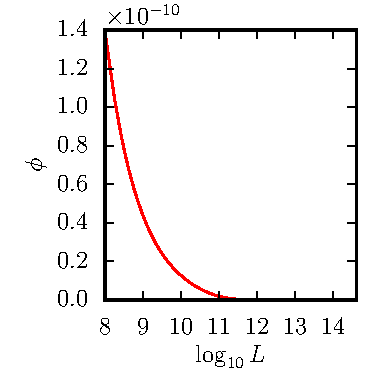
\includegraphics{fig/lumfunc_loglin}
		\caption{}
	\end{subfigure}
	\begin{subfigure}[c]{0.45\textwidth}
		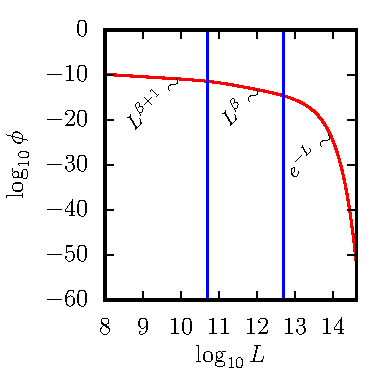
\includegraphics{fig/lumfunc_loglog}
		\caption{}
	\end{subfigure}
	\caption{Example BB1 truncated broken power law PDF, on a log-linear scale (a) and on log-log scale (b), with parameters $(l,u) = (5\times 10^{10}, 5\times 10^{12})$ in dimensionless units, and $\beta = -1.5$.
	In Panel~b the blue verticals show the lower limit $l$ and upper limit $u$ of the region where the power law slope is $\approx\beta$.}
	\label{fig:lumfunc}
\end{figure}

We simulate observations of a population described by the BB1 model, with parameters chosen so that galaxies with $L>l$ have a distribution similar to that found in the analysis by Blanton et al. (\citealt{blanton2003galaxy}, B03) of $\approx 150,000$ galaxies with spectroscopic redshifts observed in the Sloan Digital Sky Survey (SDSS).
We set $u = 1\times 10^{10} L_\odot$ (where $L_\odot$ denotes the solar luminosity; this is approximately equal to the B03 value of $L_*$ in a Schecter function fit), $\beta = -1.5$ (a bit steeper than the B03 value), and $l= 1\times 10^{8} L_\odot$, corresponding to the lowest luminosities studied by B03.
We choose survey parameters corresponding to a deeper survey than SDSS, thus probing luminosities dimmer than $L=l$.
These choices are motivated in part by current and emerging surveys, such as the photometric (broad-band) surveys by the Panoramic Survey Telescope and Rapid Response System (Pan-STARRS, current) and the Large Synoptic Survey Telescope (LSST; starting in 2023),   and the spectroscopic (redshift) survey by the Dark Energy Spectroscopic Instrument (DESI; starting in 2019).

For distances, we sample values from a spatially homogeneous population extending out to a maximum distance $\rmax = 1$~Gpc.
Only very luminous sources can be detected from large distances.
For the detection criteria we adopt (see below), this maximum distance is such that galaxies are visible beyond $\rmax$ only if $L \gtrsim 20u$, an event with negligible probability (which we formally exclude by truncation).

% suppression factor  $e^{-20} \sim 2\times 10^{-9}$

% This appears to be an implementation detail: don't bother sampling L's you know you'll reject
% \enote{Janos also truncated below $l$; is this necessary?}

The upper luminosity scale, $u$, and maximum distance, $\rmax$, together define a fiducial flux value,
\begin{equation}\label{eq:Ffid}
\Ffid
  \equiv \frac{u}{4\pi r_{\rmax}^2} 
  \approx 3.2\times 10^{-13} \left(\frac{u}{10^{10} \Lsol}\right)
      \left(\frac{\rmax}{1~\text{Gpc}}\right)^{-2}\;
      \text{erg cm$^{-2}$ s$^{-1}$}.
\end{equation}
This is a convenient unit in which to express fluxes.
Although $\Ffid$ is minuscule, modern survey telescopes would detect $\sim 10^4$ to $10^5$ photons from a source with this flux.

% TODO:  Double-check this:
%\enote{Note the parameter value changes!  
%The plots need revision; luminosity axis labels need to be shifted by $\times 100$, and the axis label should read $\log_{10}(L/L_\odot)$.  
%Check the $\rmax$ value and make sure it corresponds to the flux limit and luminosity truncation after shifting to the new params.}

Now we consider the choice of prior for the population parameters.
For $\beta$, we adopt a prior that is flat with respect to the angle in $\log$-$\log$ space.
This choice has the virtue of not putting a lot of prior probability on the steep slope range, which a flat prior on $\beta$ would do.
Denoting the angle by $\varphi$, if we adopt a prior PDF of $g(\varphi)$ on $\varphi$, the prior on $\beta = \tan\varphi$ is $p(\beta) = g(\varphi)/(1 + \beta^2)$.
For a flat $\varphi$ prior between two cut-offs $\varphi_L$ and $\varphi_U$,
\begin{equation}
	p(\beta) = \frac{1}{\varphi_U - \varphi_L} \cdot \frac{1}{1 + \beta^2}.
\end{equation}
This is a truncated Cauchy distribution.
The BB1 distribution requires $\beta > -2$, corresponding to $\varphi_L = -1.107$.
If we require Eq.~\ref{eq:lumPDF} to be decreasing, the upper limit becomes $\beta < 0$, corresponding to $\varphi_U = 0$.
Thus, the prior on $\beta$ is
\begin{equation}
p(\beta) = \frac{0.903}{1 + \beta^2} \quad \quad \quad \textrm{for} -2 < \beta < 0.
\end{equation}
For the upper scale we use a log-flat prior, a conventional choice for a scale parameter that must be positive, even though this will be improper on both sides, we can ignore the impropriety and the normalizing constant since the likelihood function will make the posterior proper.
A prior flat in $\log{u}$ corresponds to $p(u) \propto \frac{1}{u}$.
The lower scale $l$ must be below the upper scale $u$, which we can ensure by using a prior factored as $p(l, u) = p(u) p(l \assm u)$ and taking $p(l \assm u)$ to vanish for $l \geq u$.
A log-flat prior also seems appealing for $l$ but the data (i.e. luminosity measurements) do not probe the distribution down to zero due to the flux limit of the telescope, we could not have a proper prior without introduction a lower cut-off.
Instead, we simply use a flat prior on $l$.
Hence, the overall prior will be \begin{equation}\label{eq:popParsPriorPDF} p(\beta, l, u) \propto \frac{l}{u \cdot (1 + \beta^2)} \quad\quad\quad \textrm{for} -2 < \beta < 0, l < u.
\end{equation}

%................................................................................
\subsection{Simulation setup: detection and measurement}
\label{sec:simsetup-data}

We simulate measurement errors and selection effects using a simplified model commonly adopted in astronomical simulation studies (\citealt{F99-SDSSSim,LSSTRefDesign}).
Modern astronomical optical detectors, such as cameras using charge-coupled devices (CCDs), count photons.
The Poisson distribution accurately describes photon arrival and detection, but there are additional contributions to measurement uncertainty, including from backgrounds and electronic noise.
To screen out false detections, only reasonably strong candidate sources are accepted as genuine, so that catalog data are typically in the large-counts regime.
Simulation models work in this regime, approximating the Poisson distribution by a normal distribution, and treating the additional contributions to measurement uncertainty also using normal distributions.
The overall measurement uncertainty thus is approximately normal, with a variance found by adding the variances of the component processes.

For simulation studies of hierarchical Bayes approaches, it is important to distinguish approximations of the sampling distribution used to generate simulated data, and approximations of the member likelihood functions needed for inference with a particular simulated dataset.
As a concrete illustration of the distinction, consider a source with true flux $F$ being measured by an idea photon counting detector, with measurement uncertainty due only to Poisson counting uncertainty associated with the source flux.
For an instrument with projected area $A$ observing for a time $T$, the expected number of photons is $\mu = ATF$, and the standard deviation in the number of photons is $\mu^{1/2}$.
In the high-counts regime, we could simulate an observation by drawing a number of photon counts, $n$, from a normal distribution $N(\mu,\mu)$, i.e., with
\begin{equation}\label{eq:PoissonNormal}
p(n|F) \approx \frac{1}{(ATF)^{1/2}\sqrt{2\pi}}
  \exp\left[-\frac{(n-ATF)^2}{2ATF}\right].
\end{equation}
Suppose the simulated value of $n$ is $n_{\rm obs}$.
For analysis of that observation, we would need to approximate the member likelihood function based on that datum.
The exact likelihood function, $\mlike(F)$, based on the Poisson sampling distribution, is proportional to a gamma distribution with shape parameter $\alpha = n_{\rm obs} + 1$ and scale parameter $1/AT$, with its mode at $\hat{F} = n_{\rm obs}/(AT)$, which could serve as a convenient point estimator.
Expressed in terms of $\mu = ATF$, this gamma distribution has mean $\langle ATF\rangle = n_{\rm obs} + 1$ and variance $n_{\rm obs} + 1$.
For large $n_{\rm obs}$, the member likelihood function is thus well approximated by a Gaussian function with mean and variance equal to $n_{\rm obs}+ 1 \approx n_{\rm obs}$:
\begin{align}\label{eq:GammaNormal}
\mlike(F) 
  &\propto \frac{1}{n_{\rm obs}^{1/2}\sqrt{2\pi}}
     \exp\left[-\frac{(ATF - n_{\rm obs})^2}{2n_{\rm obs}}\right]\nonumber\\
  &\propto \exp\left[-\frac{(F - n_{\rm obs}/(AT))^2}
     {2n_{\rm obs}/(AT)^2}\right].
\end{align}
Thus for generating simulated data, we would use a normal distribution, (\ref{eq:PoissonNormal}), with variance depending on the true flux.
But for analyzing a simulated data set, we would use likelihood functions proportional to normal distributions, 
(\ref{eq:PoissonNormal}), with variances depending on the simulated data, $n_{\rm obs}$, for each object.

For our simulations of catalog data, we use normal sampling distributions for estimated fluxes, $\Fhat_i$, with standard deviations that depend on the true fluxes, $F_i$, according to
\begin{align}
\sigma(F)
  &= \sqrt{\sigma_0^2+(\alpha F)^2}\nonumber\\
  &= \sigma_0 \left[1 + \left(\frac{\alpha F}{\sigma_0}\right)^2 \right]^{1/2},
\label{eq:sig-F}
\end{align}
where $\sigma_0$ characterizes the noise contributions from backgrounds and detector electronics, and $\alpha$ characterizes how Poisson fluctuations in the number of detected photons influence $\Fhat_i$, relative to the flux-independent noise sources.
For an object with simulated best-fit flux $\Fhat_i$, we use a member likelihood function that is a Gaussian function with mode at $\Fhat_i$ and standard deviation parameter
\begin{equation}
\hat{\sigma}(\Fhat_i)
  = \sqrt{\sigma_0^2+(\alpha \Fhat_i)^2},
\label{eq:sig-Fhat}
\end{equation}
using the same values for $\sigma_0$ and $\alpha$ as are used for the sampling distributions.
Based on published simulations of existing and anticipated surveys (\citealt{F99-SDSSSim,LSSTRefDesign}), we set $\alpha = 10^{-2}$ for our simulations.
We set $\sigma_0 = 6.4\times 10^{-10}$ and $\alpha = 10^{-2}$ and \mbox{$\sigma_0 = 6.4\times 10^{-10}$~erg~cm$^{-2}$~s$^{-1}$} for our simulations.
The latter value was chosen so that sources with $L=20 u$ at $r=\rmax$ are just detectable by the error-based detection criterion described below.


% Checked by Janos 4/9/17:
% \enote{Check these error/threshold params; they should correspond to Janos's values shifted to physical units.}

For detection, we require a candidate object to have estimated flux a factor $\nu = 5$ times the measurement error.
This corresponds to a threshold flux satisfying $\Fth = \nu \hat{\sigma}(\Fth)$, which gives
\begin{equation}\label{eq:Fth}
\Fth = \frac{\nu \sigma_0}{\sqrt{1-\alpha^2}}.
\end{equation}
For the parameters of our simulation, this corresponds to \mbox{$\Fth \approx 3.2 \times 10^{-9}$~erg~cm$^{-2}$~s$^{-1}$}.
The detection efficiency is the probability that the measured value, $\Fth$, for a source with true flux $F$ will be above the threshold,
\begin{align}\label{key}
\eta(F)
  &= p(\Fhat > \Fth|F)\nonumber\\
  &= \Phi\left(\frac{F - \Fth}{\sigma(F)}\right),
\end{align}
where $\Phi(\cdot)$ denotes the standard normal cumulative distribution function.



%-------------------------------------------------------------------------------
\iffalse
\subsection{Simulation setup}
\label{sec:simsetup}


\enote{IGNORE THIS SUBSECTION.}


In case of real measurements the distance of the objects is known from redshift observations.
In our simplified case we assume these distance measurements to be without error.
To compile the simulated data set, we assume a spherically symmetric, homogeneous distribution of galaxies and generate the random distances $r_i$ accordingly.
We use the inverse-square law
\begin{equation}
F_i = \frac{L_i}{4 \pi r_i^2}.
\end{equation}
The observational noise $E$ of the flux $F$ is modeled as Gaussian with zero mean and a standard deviation of
\begin{equation}
\sigma(F)=\sqrt{\sigma_0^2+(0.01F)^2}.
\label{eq:error}
\end{equation}
The flux limit of the telescope is the constant $T$ and $C$ will denote the event when an object is detected, i.e. the noisy flux is above the threshold: $D > T$.
When generating the random sample, the luminosity is limited between $10 \leq \log_{10}{L} \leq 14$ which implies the distance limit
\begin{equation}
r_\textnormal{max} = \sqrt{\frac{L_\textnormal{max}}{4 \pi T}}.
\end{equation}

As it was discussed above in Sec.~\ref{sec:intro}, the spatial distribution of galaxies is considered homogeneous, hence the density function becomes \begin{equation}\label{eq:dist_dens_func}
\delta(r) = 
\begin{cases} 
    \dfrac{3r^{2}}{r_{\max}^{3}} & \quad \text{if } 0\leq r\leq r_{\max}\\
    0 & \quad \text{otherwise}
\end{cases} 
\end{equation}
and the cumulative distribution function: \begin{align}\label{eq:dist_cum_func} \Delta(r)= \begin{cases} 0 & \quad \text{if } r<0\\ \dfrac{r^{3}}{r_{\max}^{3}} & \quad \text{if } 0\leq r\leq r_{\max}\\ 1 & \quad \text{if } r\geq r_{\max} \end{cases} \end{align}


To take the selection effect of the flux limit into account, we have to calculate the probability of measuring a galaxy with a given luminosity and distance above the flux limit.
By assuming Gaussian noise, as we already did in Sec.~\ref{sec:bb1truncpl}, the sought probability becomes
\begin{align}
p(C | L, r) &= p(C | F) = \Pr(D>T | F)\\
&= \Pr(F+E>T)\\
&=\Pr(\underbrace{F + E}_\text{$\sim \mathcal{N}\left(F,\sigma(F)\right)$} > T)\\
&=\frac{1}{2}\left( 1 + \erf\left( \frac{F - T}{\sqrt{2}\sigma(F)} \right) \right)\\
&=:\zeta(F ; T,\sigma_0)
\label{eq:pclr}
\end{align}
\fi


%................................................................................
\subsection{Case study}

We apply the hierarchical Bayesian model to estimate the model parameters of a simulated random sample of $100{,}000$ galaxies.
We compare the results of the Bayesian analysis to maximum likelihood and evaluate the performance of the GPU-based implementation.
The true values of the population parameters are listed in the first row of Tab.~\ref{tab:sum_est}.

We executed 1.5M burn-in steps and the same number of live MCMC steps to sample the probability distribution of the population parameters.
The length of the burn-in sequence was chosen based on visual inspection of the autocorrelation plots.
To reduce autocorrelations in the Markov chain, $\theta$ samples were thinned and only every $150^\textnormal{th}$ sample was kept, hence the final number of samples was $10{,}000$.
Fig.~\ref{fig:results} shows the traces, histograms and autocorrelation plots of the population parameters whereas Tab.~\ref{tab:sum_est} lists the result in a numerical format.

% This uses Janos's original dimensionless units:
%\begin{table} \begin{center} \begin{tabular}{ l | d{12} | d{12} | d{12} | } \cline{2-4} & \beta & l & u \\ \hline \multicolumn{1}{|l|}{$\theta_\text{true}$} & -1.5 & 5.0\hphantom{000} \times 10^{10} & 5.0\hphantom{000} \times 10^{12} \\ \hline \multicolumn{1}{|l|}{$\theta_{\text{MCMC}}$} & -1.5037 & 5.0302 \times 10^{10} & 5.0000 \times 10^{12} \\ \hline \multicolumn{1}{|l|}{$\sigma_{\theta\text{,MCMC}}$} & 0.0059 & 3.3548 \times 10^{9} & 3.1806 \times 10^{10} \\ \hline \multicolumn{1}{|l|}{$\theta_{\text{MLE}}$} & -1.5564 & 7.3222 \times 10^{10} & 5.7207 \times 10^{12} \\ \hline \multicolumn{1}{|l|}{$\theta_{\text{MLE, no noise}}$} & -1.5009 & 4.9341 \times 10^{10} & 4.9819 \times 10^{12} \\ \hline \multicolumn{1}{|l|}{$\lvert \theta_{\text{true}} - \theta_{\text{MLE}} \rvert$} & >9.5525 \cdot \sigma_{\beta\text{,MCMC}} & >6.9221\cdot\sigma_{l\text{,MCMC}} & >22.6591\cdot\sigma_{u\text{,MCMC}} \\ \hline \end{tabular} \end{center}\end{table}

\begin{table}
\begin{center}
\begin{tabular}{ l | d{12} | d{12} | d{12} | }
\cline{2-4}
  & \beta & l & u \\
\hline
 \multicolumn{1}{|l|}{$\theta_\text{true}$} & -1.5 & 1.0\hphantom{000} \times 10^{8} & 1.0\hphantom{000} \times 10^{10} \\
\hline
  \multicolumn{1}{|l|}{$\theta_{\text{MCMC}}$} & -1.5036 & 0.99574 \times 10^{8} & 0.99962 \times 10^{10} \\
\hline
  \multicolumn{1}{|l|}{$\sigma_{\theta\text{,MCMC}}$} & 0.0059 & 6.8 \times 10^{6} & 6.36 \times 10^{7} \\
% \hline
%  \multicolumn{1}{|l|}{$\theta_{\text{MLE}}$} & -1.5564 & 1.46444 \times 10^{8} & 1.14414 \times 10^{10} \\
% \hline
%  \multicolumn{1}{|l|}{$\theta_{\text{MLE, no noise}}$} & -1.5009 & 0.98682 \times 10^{8} & 0.99638 \times 10^{10} \\
% \hline
%  \multicolumn{1}{|l|}{$\lvert \theta_{\text{true}} - \theta_{\text{MLE}} \rvert$} & >9.5226 \cdot \sigma_{\beta\text{,MCMC}} & >6.8309\cdot\sigma_{l\text{,MCMC}} & >606.4789\cdot\sigma_{u\text{,MCMC}} \\
\hline
\end{tabular}
\end{center}
\caption{Summary of parameter estimation results.
The first row of the table indicates the true values used to simulate data.
The second row lists posterior means, and the third row lists posterior standard deviations (both estimated using the MCMC output).
% For reference, we indicate the outcome of the ML estimatior run on the simulated data with and without noise in rows 4~and~5, respectively.
% To compare the Bayesian model to ML, the last row of the table shows the difference between the ML estimator and the true values in terms of the standard deviation of the posterior from the Bayesian model.
} \label{tab:sum_est} \end{table}

\begin{figure}
    \centering
    \begin{subfigure}{0.3\textwidth}
        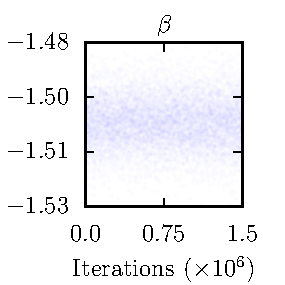
\includegraphics{{fig/beta}}
    \end{subfigure}
    \begin{subfigure}{0.3\textwidth}
        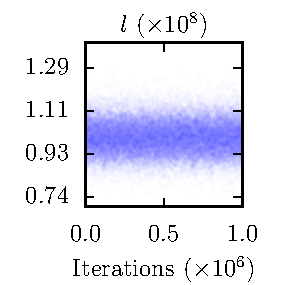
\includegraphics{{fig/lowerscale}}
    \end{subfigure}
    \begin{subfigure}{0.3\textwidth}
        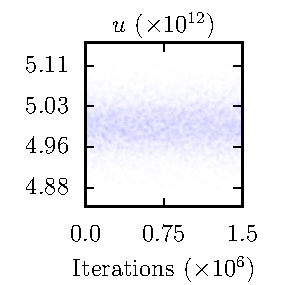
\includegraphics{{fig/upperscale}}
    \end{subfigure}
    
    \begin{subfigure}{0.3\textwidth}
        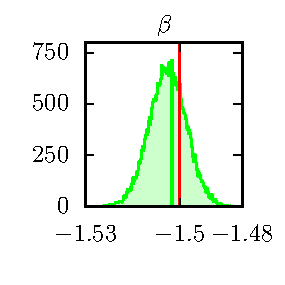
\includegraphics{{fig/beta_histo}}
    \end{subfigure}
    \begin{subfigure}{0.3\textwidth}
        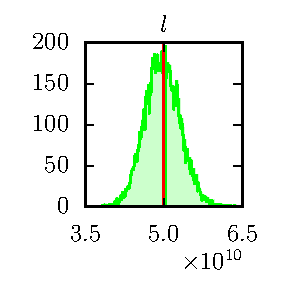
\includegraphics{{fig/lowerscale_histo}}
    \end{subfigure}
    \begin{subfigure}{0.3\textwidth}
        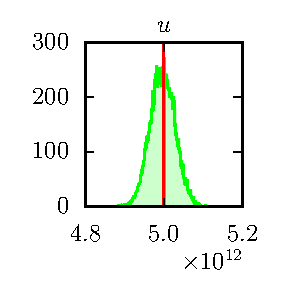
\includegraphics{{fig/upperscale_histo}}
    \end{subfigure}    
    
    \begin{subfigure}{0.3\textwidth}
        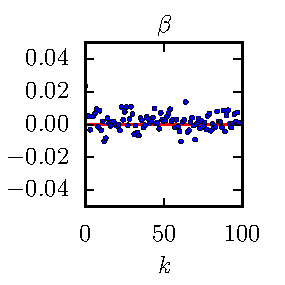
\includegraphics{{fig/autocorr_beta}}
    \end{subfigure}
    \begin{subfigure}{0.3\textwidth}
        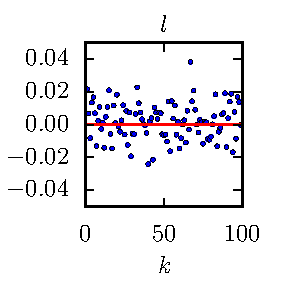
\includegraphics{{fig/autocorr_lowerscale}}
    \end{subfigure}
    \begin{subfigure}{0.3\textwidth}
        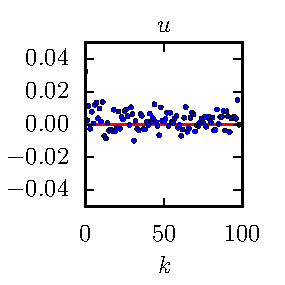
\includegraphics{{fig/autocorr_upperscale}}
    \end{subfigure}    
    \caption{Trace (upper row), histogram (middle row) and autocorrelation (lower row) plots of MCMC posterior samples of the three population parameters; $k$ is the lag for the autocorrelation. The red vertical lines on the histograms show the true values of the parameters.}
	\label{fig:results}
\end{figure}

%................................................................................
\subsection{Performance tests}

\begin{figure}
   	\begin{center}
   		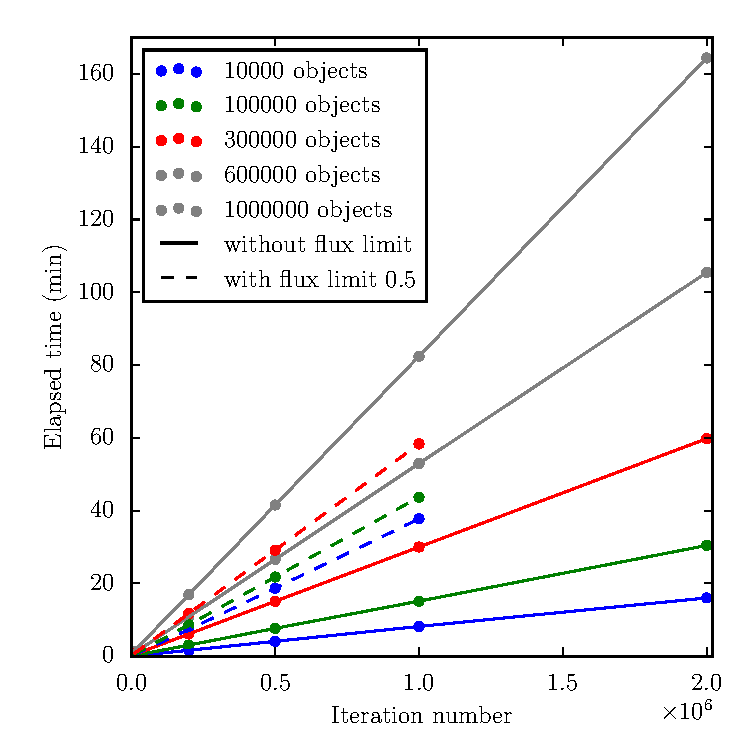
\includegraphics{{fig/performance_iter_vs_time}}
   	\end{center} 
    \caption{Runtime of CUDAHM code as a function of iterations for different numbers of objects, for models with (solid lines) and without (dashed lines) thinning corresponding to an observed flux threshold.}
    \label{fig:performance_iter_vs_time}
\end{figure}

\begin{figure}
   	\begin{center}
   		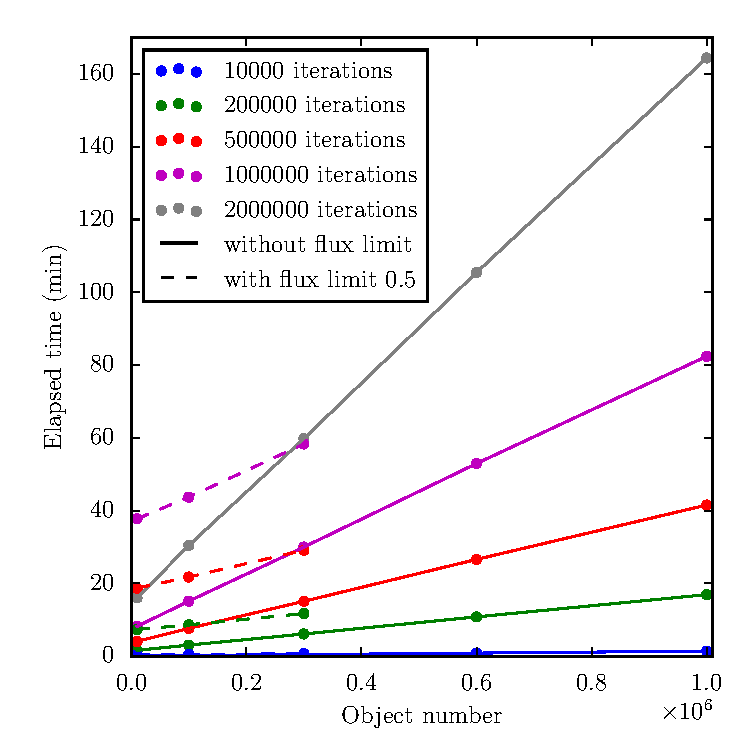
\includegraphics{{fig/performance_obj_vs_time}}
   	\end{center} 
    \caption{Runtime of the GPU code as a function of the number of objects, after a given number of iterations, for models with (solid lines) and without (dashed lines) a detection threshold. Including a threshold results in an approximately fourfold increase of runtime. The scaling of runtime with the number of objects is approximately linear.}
    \label{fig:performance_obj_vs_time}
\end{figure}

% TODO:  Eliminate 0.5 from legend; "flux threshold"

% TODO:  Sort out threshold computational cost.
% *** \enote{Clarify computational expense associated with normalization integral.  It seems not correct; the normalization should be a fixed cost, independent of object number.}

% TODO:  Is the linear scaling any different for a non-GPU implementation?

We used NVIDIA Tesla K40c cards for performance tests.
First, we executed tests without imposing a flux limit, which is a much simpler case as it does not contain the time-consuming numerical integration in the denominator of Eq.~\ref{eq:epdf}.
Next, we performed calculations incorporating the flux limit.
Fig.~\ref{fig:performance_iter_vs_time} shows the elapsed time as a function of iteration number (non-thinned) for different number of objects.
The functions are essentially linear as iteration steps always take a fixed amount of time.
More informative is Fig.~\ref{fig:performance_obj_vs_time} where we plot the elapsed time as a function of the number of objects for various numbers of iteration steps.
The linear scaling of computation time with the number of objects is due to the fact that the latent characteristics are conditionally independent, so that their sampling step in the MWG algorithm does not depend in a complicated way on the size of the latent parameter space.
As it is visible from the figures, incorporating a threshold introduces a significant (but fixed) factor in the computational expense.

% Real galaxy catalogs contain objects on the order of $10^8$, two magnitudes more than our simulated data set.
% Extrapolating from out performance numbers, estimating the parameters of the luminosity function with $2 \times 10^5$ Markov steps would take about 2000 minutes, a bit less then one and a half days, which makes applying our method to real data feasible.

Current astronomical catalogs for which the type of parametric modeling presented here is appropriate range in size from hundreds to well over $10^6$ objects.
Forthcoming catalogs will contain of order $10^8$ or more objects.
The example presented here shows that GPU-accelerated hierarchical Bayesian inference is feasible for such catalogs.
E.g., scaling from the BB1 example here, parametric inference with models with several parameters, for catalogs with $\sim 10^8$ objects, should be achievable with computing times of order a day with modest-sized clusters of GPUs.
